\section{Problem}

The Medical test Records project approaches two main issues that hospital information systems face. \\

The first issue, is controlling access to a patient's profile.
A patient's profile has associated with it a group of information with different levels of sensitivity, such as age, name, blood type, diseases, family records and others.
A patient's name is not extremely sensitive so most employees can access it. However, for instance,the patient's family records do not need to be accessed nor should be accessible to most of the hospital staff, for example to volunteers. \\

Given this scenario, the access control mechanism must be able to correctly determine, and enforce the correct policies so that different parts of a patient's profile are only available to whom actually requires them to fulfill one's obligations to the patient, regarding the performed role and in the correct context. \\

The second problem comes from medical tests being analyzed in different facilities, like partner labs, that are not part of the hospital infrastructure, but require that both are interconnected in a way that enables all sides to identify each other and communicate in a secure way. \\

\subsection{Requisites}

Given the previous problems, the implementation of this project requires the following security guarantees:
\begin{itemize}
	\item A fine grained access control and secure authentication mechanism.
	\item Authenticity of all communications with the information systems.
	\item Confidentiality of all communications with the information systems.
	\item Integrity of all communications with the information systems.
	\item Non-repudiation of the communications with the partner labs.
\end{itemize}

\subsection{Trust assumptions}


There are three main entities in this project:\\
\begin{itemize}
	\item The Hospital System
		\subitem The system that will store all the patient data and tests results received from the labs.
	\item The Partner Labs System
		\subitem The partner lab can be internal, or external to the Hospital network. The internal lab is in the same network as the Hospital, but as the external lab, they will have different infrastructures from the hospital, which means they will have their own certificates and machines.
	\item The users of those systems, the staff.
	\item The certificate authority.
\end{itemize}


In case of the staff there is a full trust assumption that they won't have their credentials stolen, shared or compromised in any way, and as such we will not provide any mechanism to rapidly revoke those credentials. \\

Regarding the certificate authority, there is a full trust assumption that the private key used to issue/sign certificates won't be stolen and as such, we won't have a mechanism to revoke certificates. \\

Concerning the access control components which will be explained further (PDP,PEP...), there is a full trust assumption that those components will be correctly and logically well implemented, and won't allow any type of unauthorized access. \\

All communications with the partner labs (internal or external) will use HTTP requests with a custom security protocol, and will be considered secure and resistant against attacks like replay, tampering and eavesdropping. \\

There is also a full trust assumption, that all the libraries and frameworks used are error free and won't give any type of access to an attacker. \\


\section{Proposed solution}

\subsection{Overview}

The implementation will be separated in two main components, an hospital REST API\cite{springmvc} and a laboratory REST API, which will act as client or server, depending on the action being done. When further mentioned API in this text, both the hospital's API and lab's API's are being referred to, as they will be pretty similar in terms of security and access control. The only difference between those two entities (hospital and labs) API's, are the possible actions and data stored. \\

All the components involved in this project, will be developed using the Java\cite{java} programming language. \\

All requests received by the API need to possess a proof of identity to be further processed (accept or refuse action), in this case will be a token provided by the respective entity API, after authentication using the correct set of credentials (username:password). The token is transported in the "Authorization" header of the HTTP request. If the token is not present the request will be refused with status code 401 UNAUTHENTICATED. \\

The database will store the hash version of the password using the Bcrypt\cite{bcrypt} algorithm, which already salts the passwords. The API will validate the received credentials by hashing them and comparing to the value already stored in the database. Further steps can be taken to protect against brute-force attacks like increasing the processing time or limiting the number of login attempts, which will only be implemented in the advanced version of the project if there is time. \\


If the request contains all necessary information (access token), it will be forwarded to the access control mechanism. \\

The access control mechanism is composed by 4 major components:
\begin{itemize}
	\item PEP - Policy Enforcement Point
	\item PDP - Policy Decision Point
	\item PAP - Policy Administration Point
	\item Policy Store
\end{itemize}

The PEP will send a XACML\cite{xacml} request to the PDP, the PDP will then based on the policies defined by the system return a XACML response which will dictate the action (ACCEPT or REFUSE) that PEP will enforce. If the result is ACCEPT, the request will continue and read or write the requested resource, otherwise the request will be dropped and replied with a 403 UNAUTHORIZED.

	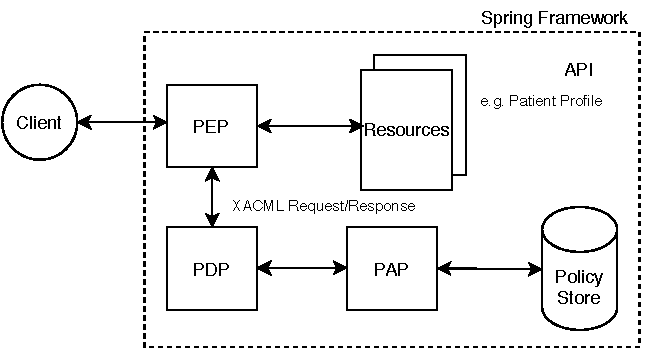
\includegraphics[width=.6\textwidth]{figs/access_control.pdf}


The PEP will be  contained on the API on the hospital's server and the rest of the components will be on a separate machine.

\subsection{Deployment}
The following figure includes the distinct machines of this system, and as mentioned they will be interconnected through secure channels (TLS or custom protocol).

	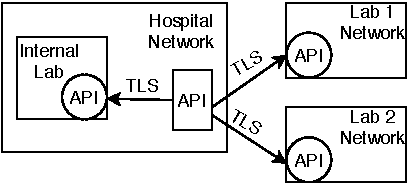
\includegraphics[width=.4\textwidth]{figs/infrastructure.pdf}

The partner lab staff will send HTTP requests to their API which in turn will communicate with the Hospital API using the custom protocol to send and receive any data related to the tests data.

The deployment scripts will use Vagrant\cite{vagrant} to manage and deploy the VM's with the correct network configurations and all the necessary software to run the applications. \\

In this project there will be used only one external lab, but thats only for ease of management, as adding more lab's is just a matter of editing the deployment scripts. Also, in the diagram where there is an API circle, there are actually two machines, one with the main API and PEP and the other with the rest of the access control components (PDP,PAP...).


\subsection{Secure Channels}

All communications between the end-users (staff) and respective API's will run with TLS to provide confidentiality, integrity and freshness. TLS, between those entities will be provided by the Spring framework\cite{springmvc}, which is the framework and language that will be used to develop the project. And using the Diffie-Hellman protocol for key exchanging. \\

The communications between the Hospital API and partner lab API will be under a custom made protocol which will provide the same properties as the TLS channel (confidentiality, integrity and freshness). \\
	
The secure channels will require the definition of a certificate for each entity, we will consider that the certificates are installed manually by an administrator on each respective machine.
We will have a made-up CA, which we will use to issue and sign the hospital and lab's certificate (including labs inside the hospital)(certificates created with OpenSSL\cite{openssl}). Those certificates alongside with the secure communication channel, will be used to digitally sign the sent tests data to guarantee its authenticity at any time.
In order to validate the certificate received by the server during the TLS Handshake, each machine will have the root CA certificate already installed, manually, by an administrator.\\ 
 
\subsection{Secure Protocol to Develop}
The custom secure protocol will enable secure communications between the Hospital API and partner lab, providing the same properties as TLS.
The protocol will require a TCP listener socket in the receiving machines (e.g. 1443) and await for requests, meanwhile all new communications will start from a random unprivileged port (greater than 1024) in the request machine. The initial part of the protocol will require an handshake where the transmissor will start by sending an "HELLO" message to the receiver. The receiver will answer with its own certificate and chosen cipher suite (e.g. TLS\_ECDHE\_RSA\_WITH\_AES\_128\_GCM\_SHA256).

In our case there will be only one cipher suite, the protocols to be used will be RSA for key exchanging, AES-256 for block cipher and hmac-sha256 for message authentication.

After receiving the certificate, the client will verify it by checking its hostname (verify if it really is the server), expiration date and its validity with the CA. If it's all ok, the client will generate a pseudo-random secret (random byte string), encrypt it with the receiver/target public key and send it back. From that secret, both client and server will generate session keys. To check if all went ok during the handshake they both will send a "Finished message" to each other, if both can decrypt it, communications can start. For extra security the "finished" message could be the hash of all exchanged messages to avoid tampering. All previous mentioned messages will also have a nonce and a timestamp for freshness. \\


\section{Plan}

\subsection{Basic}
\begin{itemize}
	\item API.
		\subitem The following endpoints will exist in the API:
		\subitem - GET /patient/{id}/name, returns the name of the patient with id {id}.
		\subitem - GET /patient/{id}/diseases, returns the diseases the patient has (e.g. tuberculosis...)
		\subitem - GET /patient/{id}/treatment, the necessary treatment (e.g. what medicine the patient needs, 500mg of Vicodin).
		\subitem - GET /patient/{id}/testsresults, the results of the tests.
		\subitem - POST /testresults/{id}, used by the partner labs to write the tests results.
	\item TLS for secure communication channels with the end-users.
	\item Access Control.
		\subitem The following roles will exist: Doctor, Nurse, Janitor and Lab Employee. The doctor role will give read access to any information about the patient, the nurse role will give read access to any information regarding the necessary treatment (e.g. food, medicine...), the janitor role will only give  read access to superficial information like the patient name, finally the lab employee won't have access to any patient profile information, they can only see in their entity respective API if there is any requests from the hospital to process tests data and writing the results of the tests data.
	\item Custom communications protocol. (Hospital - Partner lab's).
\end{itemize}

It is expected that this version will take around 2 weeks to complete. 


\subsection{Intermediate}
\begin{itemize}
	\item The necessary mechanism to check tests data authenticity at any time. (Digital Signature)
	\item Sensitive information like passwords stored in a safe way using Bcrypt (already salts).
	\item Finishing the implementation of the custom communications protocol
\end{itemize}

This phase should take around 2 week's.


\subsection{Advanced}
\begin{itemize}
	\item Encryption of all the confidential information in the database, to avoid leaks in case of a breach.
	\item Policies and authentication information cache. (Will avoid constant reads to the database everytime there is a request).
	\item Defining rule combining algorithms in the access control for  more complex decisions.
	\item Firewall implementation.
	\item Maximum number of login attempts.
	\item Finished message improved to avoid tampering during the custom protocol handshake.
\end{itemize}


\subsection{Effort Commitment}

\begin{tabularx}{0.8\textwidth} { 
  | >{\centering\arraybackslash}X 
  | >{\centering\arraybackslash}X 
  | >{\centering\arraybackslash}X 
  | >{\centering\arraybackslash}X | }
 \hline
  & Alexandru & Ana Marta & Rafaela \\
 \hline
 Week 1  & API & Deployment Scripts & Database \\
  \hline
  Week 2  & Access Control  & Custom Protocol & Tests data authenticity mechanism \\
   \hline
   Week 3  & Access Control  & Custom Protocol  & Tests data authenticity mechanism \\
    \hline
    Week 4  & Firewall  & Rule Combining Algorithms  & Database encryption \\
\hline
\end{tabularx}


\begin{thebibliography}{9}
\bibitem{springmvc} 
Pivotal Software, Spring MVC
\\\texttt{https://docs.spring.io/spring-framework/docs/3.2.x/spring-framework-reference/html/mvc.html}

\bibitem{bcrypt} 
Niels Provos and David Mazières, bcrypt
\\\texttt{https://auth0.com/blog/hashing-in-action-understanding-bcrypt}

\bibitem{xacml} 
OASIS, XACML
\\\texttt{https://www.oasis-open.org}

\bibitem{vagrant} 
HashiCorp, Vagrant
\\\texttt{https://www.vagrantup.com/}

\bibitem{openssl} 
The OpenSSL Project, OpenSSL
\\\texttt{https://www.openssl.org/}

\bibitem{java} 
Oracle, Java
\\\texttt{https://java.com/}


\end{thebibliography}

